In the above, we assumed that the parameters governing our model, $\vth=\{\alpha, \beta, \sig, \tau, \lam\}$, were known. In general, however, these parameters must be estimated from the data. Therefore, we take an approximate expectation-maximization approach for computing $\hbn$: (i) initialize some estimate of the parameters, $\hbth$, then recursively compute (ii) $\hbn$ using those parameters, (iii) update $\hbth$ given $\hbn$, and (iv) stop recursing when some convergence criteria is met.  The third step is described above; below, we provide details for each of the other steps.

\paragraph{Initializing the parameters}

Because the above model is linear, the scale of $\bF$ is arbitrary, so $\alpha$ can be fixed at $1$ without loss of generality.  The offset, however, is not arbitrary.  Because spiking is assumed to be sparse, $\bF$ tends to be around baseline, so we let $\beta$ be the mean of $\bF$.  $\sig$ is set to be the standard deviation of $\bF$.  Because previous work has shown that results are somewhat robust to minor variations in $\tau$ \cite{YaksiFriedrich06}, we initialize $\tau$ at 1 sec.  Finally, we let $\lam=10$ Hz, which is between typical baseline firing rates and evoked spike rate activity, for these data-sets.

\paragraph{Estimating the parameters given $\hbn$}

In the typical expectation-maximization setting, we find the parameters that maximize the expected value of the joint observed and hidden signals:

\begin{align} \label{eq:par1}
\hbth &= \argmax_{\bth} E_{P[\bF | \bC]} \log P[\bF, \bC | \bth].
\end{align}
In the above, however, we don't compute those expected values, rather, only the MAP estimate of the spike train and calcium trace.  Therefore, we approximate Eq. \eqref{eq:par1} by simply maximizing the parameters given the MAP estimate:

\begin{align} \label{eq:par2}
\hbth &\approx \argmax_{\bth} P[\bF| \hbC; \bth] P[\hbn | \bth]
\end{align}

%, $\hbth$, we must integrate over all possible spike trains. Unfortunately, it is not currently known how to perform this integral exactly, and approximating this integral using Monte Carlo methods is relatively time consuming (see \cite{VogelsteinPaninski09} for details).  Thus, we resort to a more drastic approximation, commonly used in state-space models.  For specifically, instead of integrating over all possibly spike trains, we only consider the most likely sequence (often referred to as the Viterbi path \cite{Rabiner89}): 
% 
% \begin{align} \label{eq:par1}
% \widehat{\bth} &= \argmax_{\bth \in \ve{\Theta}} \int P[\bF|\bC, \bth] P[\bC | \bth]  d\bC  \approx \argmax_{\bth \in \ve{\Theta}}P[\bF| \hCm, \bth] P[\hCm, | \bth]
% \end{align}
% 
\noindent where $\hCm$ is determined using the above described inference algorithm. The approximation in \eqref{eq:par1} is good whenever the likelihood is very peaky, meaning that most of the mass is around the MAP sequence.\footnote{The approximation in \eqref{eq:par1} may be considered a first-order Laplace approximation}  
%Due to the state space nature of the above model (Eqs \eqref{eq:bF} and \eqref{eq:C}), the optimization in Eq \eqref{eq:par1} simplifies significantly.  More specifically, we can write 
The argument from the right-hand-side of Eq \eqref{eq:par1} may be expanded: %written as a product of terms that we have defined in our model:

\begin{align} \label{eq:par2}
P[\bF| \hbC; \bth] P[\hbn | \bth] &= \prod_t P[F_t | \hC_t; \beta,\sig]  P[\hn_t | \lam].
\end{align}

\noindent where $\alpha$ is not present because of the arbitrary scale term, and $\tau$ is not present because it is not separable from $\hbn$. To estimate the remaining parameters, we have for $\beta$:

\begin{align}
	\hbeta &= \argmax_{\beta >0} \prod_t P[F_t | \hC_t; \beta,\sig] = \argmax_{\beta>0} \sum_t (F_t - (C_t + \beta))^2,
\end{align}

\noindent which is solved by letting $\hbeta=\langle \bF-\bC \rangle_t$, where $\langle \cdot \rangle_t$ indicates a mean over $t$.  $\sig$ is then the mean of the residuals, and $\hlam$ is the mean of $\hbn$. 
% This optimization simplifies into several separable problems.  %: (1) $\{\balpha, \beta\}$, (2) $\sig$, (3) $\gam$, and (4) $\lam$.  
% First, we solve for $\balpha$ and $\beta$.  Because solving for them jointly is non-concave, we solve for each separately.  Consider $\balpha$ only:
% 
% \begin{subequations}
% \begin{align}
% \hbalpha 
% &= \argmax_{\balpha} \prod_{t,x=1}^{T,N_p}  \p[F_{t,x} | C_t] 
% =  \argmax_{\balpha} \prod_{t,x=1}^{T,N_p} \mN(F_{x,t}; \alpha_x ( C_t + \beta), \sig^2) \\
% &= \argmax_{\balpha} \sum_{t,x=1}^{T,N_p} \log \mN (F_{x,t}; \alpha_x ( C_t + \beta), \sig^2)  \\
% &= \argmax_{\balpha}  -\frac{N_p T}{2}\log(2\pi \sig^2) -\frac{1}{2\sig^2}\sum_{t,x=1}^{T,N} (F_{t,x} - \alpha_x(C_t + b))^2 \\
% &= \argmin_{\balpha} \sum_{t,x=1}^{T,N_p} (F_{t,x} - \alpha_x(C_t + \beta))^2.
% \end{align}
% \end{subequations}
% 
% Therefore, we can solve for each of the $\halpha_x$'s separately and efficiently using Matlab's  \texttt{mldivide}: 
% %
% %\begin{align}
% 	$\halpha_x = (\bC + \beta\ve{1})\backslash \bF_x$, 
% %\end{align}
% %
% where $\bF_x=[F_{1,x}, \ldots, F_{T,x}]\T$. Given $\hbalpha$, we can estimate $\beta$:
% 
% \begin{align}
% \hbeta 
% = \argmax_{\beta>0} \sum_{t,x=1}^{T,N} (F_{t,x} - \halpha_x(C_t + \beta))^2 
% = \argmax_{\beta>0} \sum_{t,x=1}^{T,N} (F_{t,x} - \halpha_x C_t + \beta \halpha_x)^2 
% \end{align}
% 
% \noindent which can again be solved efficiently again using Matlab's \texttt{mldivide}: $\widetilde{\beta}= \halpha_x \backslash \left(\sum_{t=1}^T F_{t,x} - \halpha_x C_t\right)$.  If $\widetilde{\beta}<0$, we simply let $\hbeta=0$, else, $\hbeta=\widetilde{\beta}$.
% 
% Given $\hbalpha$ and $\hbeta$, we can now estimate $\sig$ using the residuals, i.e.,
% 
% \begin{align}
% 	\hsig^2 = \frac{1}{T N_p}\norm{\vec{\bF} - \hbalpha(\bC\T + \beta \ve{1})}^2
% \end{align}
% 
% Estimating $\lam$ is also totally straightforward: $\widehat{\lam} = \hnm' \ve{1}/ (T \Del)$. 
% % 
% % \begin{align} 
% % \widehat{\lam} &=  \frac{1}{T \Del} \hnm' \ve{1} \label{eq:lam}
% % \end{align}
% 
% We don't update $\gam$ as we have found that it does not improve inference quality (not shown), in agreement with previous work \cite{YaksiFriedrich07}.

\paragraph{Convergence criteria}

We stop iterating the parameter update whenever (i) iteration number exceeds some upper bound, or (ii) relative change in likelihood does not exceed some lower bound.  In practice, we find that parameters tend to converge after several iterations, given our initialization.  %Figure \ref{fig:spatial_EM} shows a simulation demonstrating the efficacy of this procedure.  The left panel shows the true spatial filter (top), the 1-dimensional fluorescence projection using the true spatial filter, $\bF^{opt}$ (middle), and the inferred spike train using the true parameters (bottom).  The right panel shows the estimated spatial filter, the 1-dimensional fluorescence projection using the estimated filter, $\bF^{est}$, and the inferred spike train using the estimated filter.  Note that we seeded the algorithm with the movie, and parameter estimates that were at least a factor of 2 from the true values.
% 
% \begin{figure}[h!]
% \centering 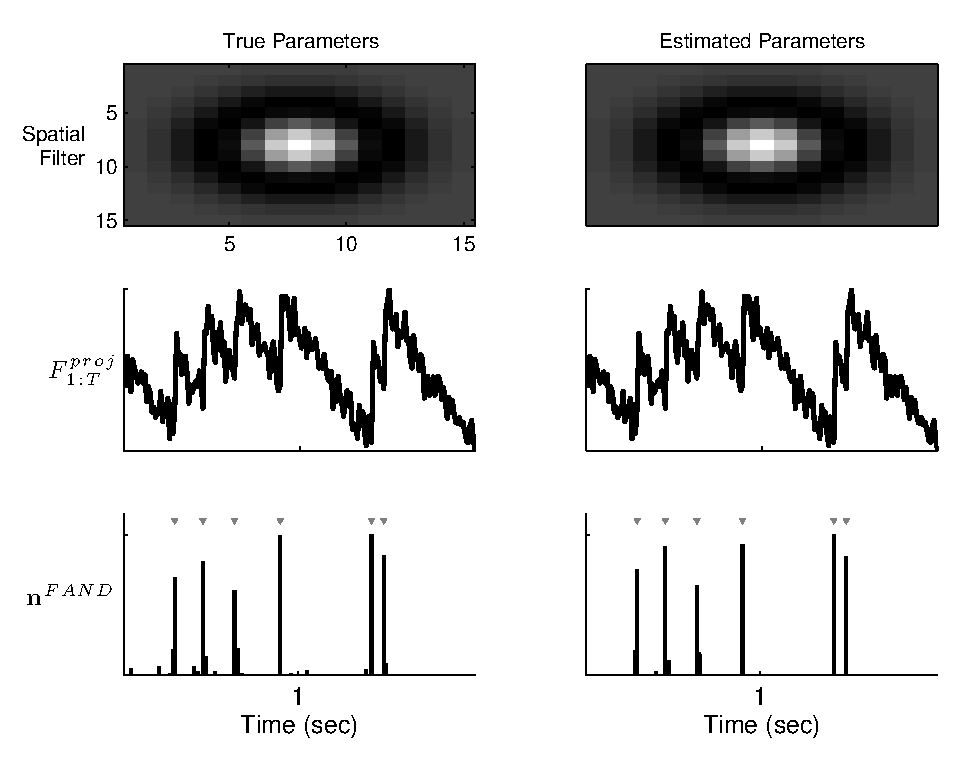
\includegraphics[width=.9\linewidth]{../figs/spatial_EM}
% \caption{A simulation demonstrating that given only the fluorescence movie, the parameters may be estimated, and the spike train inferred (c.f. Supplementary Movie 2). Top left panel: true spatial filter.  Middle left panel: projection of movie onto true spatial filter. Bottom left panel: inferred spike train using true parameters. Right panels: same as left except estimating parameters.  All parameters estimated other than $\gam$, which was assumed known.  Parameters converged within 7 iterations.  Simulation details: $T=1000$, $\Del=5$ msec, $\balpha$ is the same as in Figure \ref{fig:spatial}, $\beta=0$, $\tau=500$ msec, $\lam=10$ Hz.} \label{fig:spatial_EM}
% \end{figure}